\documentclass[10pt,conference]{IEEEtran}

\usepackage{graphicx}
\usepackage{booktabs}
\usepackage{amsmath}
\usepackage{amssymb}
\usepackage{algorithm}
\usepackage{algpseudocode}
\usepackage{subcaption}
\usepackage{multirow}
\usepackage[T1]{fontenc}

\begin{document}

\title{Classification of Network Traffic in the UNSW-NB15 Data Set Using K-Nearest Neighbours and Classification Trees}

\author{
\IEEEauthorblockN{John Oluwasegun Balogun\footnotemark[1]}
\IEEEauthorblockA{Student Number: 22677267\\
Email: 22677267@sun.ac.za}
}

\maketitle
\footnotetext[1]{Source code available at https://github.com/Noir-Cpu/cs741-assignment2.}

\begin{abstract}
Network intrusion detection relies on classification models trained to separate normal traffic from attack traffic, and the quality of the descriptive features used for training limits how reliable such a model can be. K-nearest neighbours and a classification tree respond differently to the same data-quality issues, since one classifies by distance between instances and the other by ordered threshold tests. This report investigated which of the two algorithms classified attack traffic more effectively under pre-processing matched to the distance sensitivity of each algorithm, using a version of the UNSW-NB15 network traffic data set, a data set with a severely imbalanced target class distribution. Both algorithms were tuned through a control parameter search under cross-validation, then compared under a repeated stratified partition across four performance measures. The classification tree reached a higher macro-averaged F1 score and balanced accuracy than k-nearest neighbours, a margin found to be statistically significant, while k-nearest neighbours reached a marginally higher plain accuracy. The findings indicated that the class-weighted training criterion of the tree protected the least frequent attack categories more effectively than the distance-weighted voting of k-nearest neighbours: distance weighting corrected for the proximity of neighbours, not for how often each class occurred among the neighbours found.
\end{abstract}

\section{Introduction}
\label{sec:intro}

An accurate network intrusion detection model needs descriptive features that meet an acceptable standard of data quality. An issue such as a missing value or an incompatible numeric scale degrades a trained model, and the effect depends on the classification algorithm used. This report develops two classification models, k-nearest neighbours (kNN) and a classification tree, for the attack category prediction task defined over a version of the UNSW-NB15 network traffic data set released by Moustafa and Slay~\cite{moustafa2015}. Three goals guide the study. The first goal identifies which data quality issues remain in the supplied data set. The second goal determines, separately for each algorithm, only the pre-processing transformations needed to address the identified issues; the study applies no transformation beyond what an issue and an algorithm require. The third goal determines which algorithm achieves superior classification performance once the corresponding pre-processing is applied.

The study followed a four-stage procedure. Exploratory analysis of the supplied data set quantified missing values, feature correlation, outlying values, feature scale, and class imbalance. These findings informed two pre-processing pipelines, one for k-nearest neighbours and one for the classification tree, each justified by how the algorithm is affected by a given data quality issue. A grid search under stratified five-fold cross-validation then selected a control parameter configuration for each algorithm, and the study evaluated the selected configuration under the same five-fold partition. Finally, a paired statistical test compared the cross-validated performance of the two algorithms.

The classification tree reached a mean cross-validated macro-averaged F1 score of 0.576 and a mean cross-validated balanced accuracy of 0.609, against 0.525 and 0.507 for k-nearest neighbours. This difference was statistically significant. K-nearest neighbours reached a marginally higher mean accuracy. The report identified the classification tree as the more suitable algorithm for this task, discussed further in Section~\ref{sec:results-discussion}.

The remainder of the report is organised as follows. Section~\ref{sec:background} discusses network intrusion detection as a classification problem and introduces k-nearest neighbours and the classification tree. Section~\ref{sec:methodology} reports the data quality analysis, discusses the expected impact of each issue on each algorithm, and describes the pre-processing pipeline built for each algorithm. Section~\ref{sec:procedure} describes the empirical procedure used to train and evaluate the two models. Section~\ref{sec:results} reports and discusses the results. Section~\ref{sec:conclusion} concludes the report.

\section{Background}
\label{sec:background}

This section gives background on the classification problem, then discusses the two classification algorithms under investigation. The section starts with the network intrusion detection problem, continues with k-nearest neighbours, and closes with classification trees.

\subsection{Network Intrusion Detection as a Classification Problem}
\label{sec:background-nid}

A network intrusion detection system monitors network traffic to distinguish legitimate activity from malicious activity. Moustafa and Slay~\cite{moustafa2015} created the UNSW-NB15 data set to support research into such systems. The data set combines real background traffic with synthetic attack traffic across nine attack categories: Fuzzers, Analysis, Backdoors, Denial of Service, Exploits, Generic, Reconnaissance, Shellcode, and Worms. Each record describes a single network flow through descriptive features derived from the packet headers and payload, for example the protocol type, the connection state, the number of bytes transferred in each direction, and counts of related connections in a recent time window. The classification task in this report assigns each flow to one of the nine attack categories or to the normal category, giving a ten-class supervised tabular classification problem. The classes occur at very different frequencies, a property called class imbalance. The descriptive features mix continuous, discrete count, and nominal categorical measurements at different numeric scales. These properties motivate the discussion of the two classification algorithms below, since the algorithms respond differently to skewed class frequencies, mixed feature types, and features on different scales.

\subsection{K-Nearest Neighbours Classification}
\label{sec:background-knn}

The k-nearest neighbours algorithm is an instance-based, non-parametric classification method introduced by Cover and Hart~\cite{cover1967}. The algorithm stores the full set of labelled training instances and defers computation until a new instance needs a prediction, a strategy called lazy learning. Given a query instance, the algorithm finds the k training instances nearest to the query instance under a chosen distance function, then assigns the class label that occurs most often among these neighbours. The distance function is usually a member of the Minkowski family; the Euclidean distance and the Manhattan distance are the two most common special cases. Equation~\eqref{eq:minkowski} defines the Minkowski distance between two instances represented by feature vectors $\mathbf{x}_i$ and $\mathbf{x}_j$, each of dimensionality $d$.
\begin{equation}
\label{eq:minkowski}
d(\mathbf{x}_i, \mathbf{x}_j) = \left( \sum_{l=1}^{d} |x_{i,l} - x_{j,l}|^{p} \right)^{1/p}
\end{equation}
The order $p$ sets the specific member of the family: $p=1$ gives the Manhattan distance and $p=2$ gives the Euclidean distance. Algorithm~\ref{alg:knn} gives pseudocode for classifying a single query instance with k-nearest neighbours.

\begin{algorithm}
\caption{Classification of a query instance with k-nearest neighbours}
\label{alg:knn}
\begin{algorithmic}[1]
\Require a labelled training set, a query instance, the neighbourhood size $k$, and a distance function
\Ensure the predicted class label of the query instance
\State compute the distance between the query instance and every training instance
\State select the $k$ training instances with the smallest distance to the query instance
\State count the class labels of the selected instances, optionally weighting each vote by the inverse of the corresponding distance, following the interpolation scheme of Shepard~\cite{shepard1968}
\State assign the query instance the class label with the highest vote count
\end{algorithmic}
\end{algorithm}

The value of $k$ and the choice of distance function are control parameters that set model complexity. A small $k$ gives a decision boundary that follows the training data closely and is sensitive to noise. A large $k$ gives a smoother decision boundary that risks mixing instances from different classes. Classification relies directly on distance in the original feature space, so each feature contributes to the outcome in proportion to the numeric range of that feature: a feature on a large numeric scale dominates the distance calculation unless every feature is first brought onto a comparable scale. Aggarwal et al.~\cite{aggarwal2001} showed that distance-based methods grow less discriminative as the number of feature dimensions grows, since the contrast between the nearest and the farthest neighbour of a query instance shrinks in high-dimensional spaces; this effect is called the curse of dimensionality. The number and the relevance of the supplied features therefore affect the reliability of the resulting neighbourhoods.

\subsection{Classification Trees}
\label{sec:background-tree}

A classification tree is a hierarchical, rule-based model. The tree partitions the feature space through a sequence of univariate tests, an approach developed independently by Breiman et al.~\cite{breiman1984} under the classification and regression tree framework and by Quinlan~\cite{quinlan1986} under the iterative dichotomiser framework. The tree consists of internal nodes, each associated with a test on a single feature, and leaf nodes, each associated with a predicted class label. Construction proceeds recursively from a root node containing the full training set. At each node, the algorithm evaluates every candidate feature and threshold, selects the test that gives the greatest reduction in class impurity between the parent node and the resulting child nodes, and repeats the procedure on each child node until a stopping criterion is reached. Two impurity measures are commonly used to select the test at a node $t$: the entropy in Equation~\eqref{eq:entropy} and the Gini index in Equation~\eqref{eq:gini}, where $p_{t,c}$ denotes the proportion of instances at node $t$ belonging to class $c$, and $m$ denotes the total number of classes.
\begin{equation}
\label{eq:entropy}
h(t) = -\sum_{c=1}^{m} p_{t,c} \log_2 p_{t,c}
\end{equation}
\begin{equation}
\label{eq:gini}
g(t) = 1 - \sum_{c=1}^{m} p_{t,c}^{2}
\end{equation}
Algorithm~\ref{alg:tree} gives pseudocode for the recursive construction procedure.

\begin{algorithm}
\caption{Recursive construction of a classification tree}
\label{alg:tree}
\begin{algorithmic}[1]
\Require a labelled training set at the current node and an impurity measure
\Ensure a classification tree rooted at the current node
\If{every instance at the current node belongs to the same class, or a stopping criterion is satisfied}
    \State create a leaf node labelled with the majority class of the current node
\Else
    \State evaluate every candidate feature and threshold for the reduction in impurity that the corresponding split produces
    \State select the feature and threshold that produce the greatest reduction in impurity
    \State partition the training set at the current node into child subsets according to the selected test
    \State apply the procedure recursively to each child subset
\EndIf
\end{algorithmic}
\end{algorithm}

Unlike k-nearest neighbours, a classification tree evaluates each feature independently through ordinal threshold comparisons rather than through a joint distance calculation. A monotonic transformation of a single feature therefore does not change the sequence of splits the tree selects on that feature. The depth of the tree and the minimum number of instances required at a leaf are control parameters that set model complexity. An unrestricted tree partitions the training set until every leaf is pure; this practice typically overfits the training data, whereas an excessively restricted tree underfits the training data. Quinlan~\cite{quinlan1986} showed that limiting the growth of a tree, either during construction or through later pruning, improves generalisation to instances not seen during training.

\section{Methodology}
\label{sec:methodology}

This section describes how the network traffic data set was prepared for classification and how the identified data quality issues were addressed. The section starts with the data quality issues found through exploratory analysis, continues with the expected impact of each issue on k-nearest neighbours and on the classification tree, and closes with the pre-processing pipeline built for each algorithm.

\subsection{Data Quality Assessment}
\label{sec:methodology-dq}

The data set supplied for the assignment, networkTraffic.csv, contained 257,673 instances. Each instance had forty-three descriptive features and a target feature, attack\_cat, recording the attack category. Exploratory analysis confirmed the properties stated in the assignment specification and measured the extent of each property.

Kelleher et al.~\cite{kelleher2020} distinguished two kinds of data quality issue. An issue caused by invalid data is an error, corrected regardless of the classification algorithm used afterward. An issue present in valid data is corrected only where the classification algorithm requires the correction. Every issue found through exploratory analysis was classified into one of these two categories.

The feature id is a unique record identifier. The feature took a distinct value for every instance, so the feature carried no information about the class of an instance. This issue does not depend on the classification algorithm used afterward.

The three features proto, state, and service are nominal categorical features. The feature proto recorded 133 distinct protocol values, an instance of the irregular cardinality issue described by Kelleher et al.~\cite{kelleher2020}. Three of these values, tcp, udp, and unas, accounted for the great majority of instances. The remaining values each occurred fewer than four hundred times, and several occurred fewer than 135 times.

The feature is\_ftp\_login is defined as a binary indicator. The feature took the value 2 or 4 in twenty-six instances, instead of the value 0 or 1 expected of a binary indicator, an instance of the unexpected cardinality issue described by Kelleher et al.~\cite{kelleher2020}. This report investigated the irregularity before choosing a handling strategy, rather than correcting the value on the assumption that a documented range violation is always invalid data.

The feature ct\_ftp\_cmd counts file transfer protocol commands rather than indicating a binary state. Table~\ref{tab:correlations} reported a correlation of 0.9989 between ct\_ftp\_cmd and is\_ftp\_login. On the twenty-six instances where is\_ftp\_login took the value 2 or 4, ct\_ftp\_cmd took the identical value on every instance. The two features agreed exactly on 99.997 per cent of the complete data set. The value of is\_ftp\_login on the twenty-six instances was therefore not an isolated data entry error, but a value reproduced consistently by an independently recorded feature. In practice, is\_ftp\_login was a near-duplicate count rather than a strict binary indicator, and the documented definition of the feature as binary did not hold for this data set. This report classified the issue as valid data and left the feature uncorrected: forcing the feature to a binary range would discard a value corroborated by an independent feature, with no evidence the value was recorded in error.

No feature contained a negative value, and no row duplicated another row exactly.

The feature service contained the missing value symbol \texttt{?} in 141,321 instances, 54.8 per cent of the data set. None of the remaining forty-one features contained a missing value, and the target feature contained no missing value. Kelleher et al.~\cite{kelleher2020} recommended imputation with a measure of central tendency only below a missingness rate of fifty per cent, so this rate was too high for that approach. Deletion of the affected instances was also unattractive, since these instances made up more than half of the data set.

Cross-tabulation of the missing value indicator of service against proto and against state showed a clear pattern. The proportion of missing values ranged from 100 per cent, for protocols such as arp, ospf, and gre that carry no application-layer service by construction, down to 25.7 per cent for the udp protocol. The proportion ranged from 100 per cent for several infrequent connection states down to 46.1 per cent for the CON state. The missingness of service was therefore explained by the observed values of proto and state, rather than occurring independently of these two features; Kelleher et al.~\cite{kelleher2020} termed this pattern missing at random. A missing service value means no application-layer service exists for the flow, not that a service went unrecorded. This report therefore treated the missing value symbol as valid data carrying information about the flow, rather than using model-based imputation to reconstruct information already available from proto and state.

Table~\ref{tab:correlations} listed the feature pairs with a Pearson correlation coefficient of at least 0.9 in absolute value. The pairs is\_ftp\_login and ct\_ftp\_cmd, sbytes and sloss, and dbytes and dloss correlated at 0.99 or higher, confirming the near-exact redundancy reported for the original data set. A further fifteen pairs correlated between 0.90 and 0.98, showing that groups of features recorded closely related aspects of the same network flow.

Hodge and Austin~\cite{hodge2004} identified the interquartile range rule as a standard method for detecting an outlier in a numeric feature. The interquartile range rule, applied to every numeric feature, showed that between eleven and twenty-two per cent of the instances of features such as dload, dbytes, spkts, and the connection-count features fell outside the interquartile fence. This confirmed the large positive outliers reported for the original data set. The median absolute value of every numeric feature also differed by several orders of magnitude across features: sload, recorded in bits per second, had a median absolute value near seven hundred and forty thousand, while dttl, a time-to-live count, had a median absolute value below thirty.

\begin{table}[t]
\caption{Feature pairs with Pearson correlation coefficient of at least 0.9 in absolute value}
\label{tab:correlations}
\centering
\footnotesize
\begin{tabular}{llr}
\toprule
Feature 1 & Feature 2 & Correlation \\
\midrule
is\_ftp\_login & ct\_ftp\_cmd & 0.999 \\
dbytes & dloss & 0.997 \\
sbytes & sloss & 0.996 \\
swin & dwin & 0.981 \\
dpkts & dloss & 0.980 \\
ct\_srv\_src & ct\_srv\_dst & 0.980 \\
dpkts & dbytes & 0.973 \\
spkts & sloss & 0.972 \\
spkts & sbytes & 0.964 \\
ct\_dst\_ltm & ct\_src\_dport\_ltm & 0.962 \\
ct\_dst\_src\_ltm & ct\_srv\_dst & 0.960 \\
ct\_srv\_src & ct\_dst\_src\_ltm & 0.954 \\
tcprtt & synack & 0.943 \\
tcprtt & ackdat & 0.920 \\
ct\_src\_dport\_ltm & ct\_src\_ltm & 0.909 \\
ct\_src\_dport\_ltm & ct\_dst\_sport\_ltm & 0.908 \\
ct\_dst\_ltm & ct\_src\_ltm & 0.902 \\
\bottomrule
\end{tabular}
\end{table}

Figure~\ref{fig:class-dist} showed the number of instances recorded for each of the ten target classes. The normal class and the generic attack category together accounted for a majority of the instances. The worms category had only 174 instances, a ratio of more than five hundred to one relative to the normal class. This confirmed the skewed class distribution reported for the data set.

\begin{figure}[t]
\centering
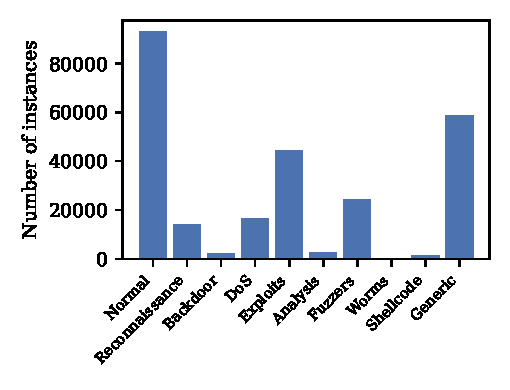
\includegraphics[width=0.85\linewidth]{../figures/class_distribution.pdf}
\caption{Number of instances recorded for each attack category in the network traffic data set.}
\label{fig:class-dist}
\end{figure}

\subsection{Expected Impact on K-Nearest Neighbours}
\label{sec:methodology-impact-knn}

K-nearest neighbours classifies a query instance using the training instances closest to the query instance under a distance function. Every data quality issue that distorts distance between instances was therefore expected to degrade classification performance.

Kelleher et al.~\cite{kelleher2020} identified a large difference in feature scale as a particular concern for a Euclidean-family distance: a feature on a large numeric range dominates the distance regardless of the relevance of the feature to the target. The scale difference between features such as sload and dttl was expected to base the resulting neighbourhood almost entirely on the largest-scale features, discarding the information in smaller-scale features, unless every feature was brought onto a comparable scale before distance was computed. The large positive outliers in features such as dload and dbytes were expected to compound this effect: a small number of extreme values inflate the numeric range of a feature, and so the influence of the feature on the distance calculation, even after linear rescaling.

The near-perfectly correlated feature pairs in Table~\ref{tab:correlations} were expected to bias the distance calculation toward the construct shared by each pair, since the same information would otherwise be counted twice in the summation of Equation~\eqref{eq:minkowski}. The presence of many correlated features was also expected to add to the input dimensionality, in line with the degradation described by Aggarwal et al.~\cite{aggarwal2001}. The high cardinality of proto, together with the nominal character of proto, state, and service, was expected to expand the input dimensionality substantially once converted to a numeric representation for distance computation, further diluting the contrast between near and distant neighbours. The missing values in service were expected to have a comparatively contained impact, provided the encoding preserved the information in these values rather than discarding more than half of the data set.

The skewed target class distribution was expected to bias a majority vote toward the frequent classes, particularly for query instances in a region of the feature space populated by more than one class. Section~\ref{sec:procedure-hyperparameters} describes a weighting scheme that gives a training instance a vote in inverse proportion to the distance of that instance from the query instance. This scheme corrects for the relative closeness of the neighbours found, but not for how frequently each class occurs among those neighbours. Where the majority class remains locally the more frequent class despite the greater proximity of a small number of minority-class neighbours, a distance-weighted vote was expected to stay biased toward the majority class. A diagnostic check supported this expectation: among the six nearest training neighbours of thirty randomly sampled worms instances, the least frequent attack category, only 15.3 per cent of the neighbours found were themselves worms instances, while 60.7 per cent were exploits instances. The neighbourhood of a typical worms instance was therefore dominated by a different attack category before any distance-based reweighting of the vote.

\subsection{Expected Impact on the Classification Tree}
\label{sec:methodology-impact-tree}

A classification tree evaluates each feature independently through a threshold comparison. The split selected on a feature depends only on the relative order of the values of that feature, not on the numeric scale. The difference in numeric scale between features, and the large positive outliers, were therefore expected to have a much smaller impact on the classification tree than on k-nearest neighbours: a monotonic transformation, including the linear rescaling that removes a scale difference, leaves the order of the values, and so the selected splits, unchanged.

For the same reason, the near-perfectly correlated feature pairs in Table~\ref{tab:correlations} were expected to have a limited impact on the classification tree. Splitting on one member of a correlated pair gives an impurity reduction closely matched by splitting on the other member, so the tree simply selects whichever feature is presented first. This differs from a distance calculation, where the duplication biases the outcome. The nominal features proto, state, and service, once converted to a numeric representation, were expected to affect the classification tree mainly through the increase in candidate splits evaluated at every node, and through the risk of a split isolating a single rare category, rather than through dilution of a distance metric.

The missing values in service were expected to affect the classification tree in the same way as k-nearest neighbours, since the information loss from inadequate treatment of these values does not depend on the classification algorithm applied afterward. The skewed class distribution was expected to bias the impurity-driven split selection of the classification tree toward the frequent classes, just as the skewed class distribution was expected to bias the majority vote of k-nearest neighbours, unless class frequencies were accounted for during training.

\subsection{Data Pre-processing for K-Nearest Neighbours}
\label{sec:methodology-prep-knn}

Guided by the expected impact discussed in Section~\ref{sec:methodology-impact-knn}, four pre-processing steps were applied before training k-nearest neighbours, and no other transformation was applied.

The feature id was removed. A unique record identifier carries no information about the class of an instance, and would otherwise add an uninformative dimension to the distance calculation.

The missing value symbol in service was replaced with a new category label, distinct from every recorded service value. The missingness mechanism established in Section~\ref{sec:methodology-dq} would otherwise favour model-based imputation, but the missing value symbol replaced the dash value used in the original UNSW-NB15 data set to mark a flow with no identified application-layer service. A category label therefore preserves exactly the same information as an imputed value, without risking the fabrication of a service value for a flow that has no service by construction. Deletion of the affected rows was rejected, since these rows make up more than half of the data set.

Consistent with the investigation in Section~\ref{sec:methodology-dq}, the values of is\_ftp\_login were left unchanged: the values outside the documented binary range were corroborated by an independently recorded feature, not indicative of a recording error.

Protocol values recorded fewer than 150 times in proto were grouped into a single \emph{other} category, reducing the cardinality of the feature from 133 to sixteen categories. Kelleher et al.~\cite{kelleher2020} associated near-singleton categories with an increased risk of overfitting: each would otherwise contribute a sparsely populated one-hot encoded dimension that dilutes the distance calculation without a reliable signal. The set of categories treated as rare was determined separately within every training fold of the cross-validation procedure described in Section~\ref{sec:procedure-cv}, so that no information about the categories in a test fold influenced the grouping applied to the corresponding training fold.

One member of each of the three most strongly correlated feature pairs in Table~\ref{tab:correlations}, namely ct\_ftp\_cmd, sloss, and dloss, was removed from the feature set, retaining is\_ftp\_login, sbytes, and dbytes respectively. A correlation of at least 0.9958 indicated the retained feature already captured the corresponding information, so the removal directly addressed the double counting described in Section~\ref{sec:methodology-impact-knn}. For the pair is\_ftp\_login and ct\_ftp\_cmd, the choice of which feature to remove was immaterial rather than evidence-driven: Section~\ref{sec:methodology-dq} reported that the two features agreed on 99.997 per cent of the instances of the data set, so is\_ftp\_login was retained arbitrarily. Feature pairs correlated between 0.90 and 0.98 were retained rather than removed. A correlation below 0.996 still allowed a measurable difference between the two features of a pair, and removing every moderately correlated feature would have risked discarding genuine, non-redundant information.

The remaining numeric features were separated into two groups by the shape of the feature distribution observed during exploratory analysis. The Fisher skewness coefficient of twenty-four features, including sbytes, dbytes, sload, dload, and the connection-count features, ranged from 1.64 for ct\_srv\_src to 78.48 for response\_body\_len. This confirmed a heavy-tailed, positively skewed distribution for each of the twenty-four features, not merely an assumption from visual inspection.

These twenty-four features were transformed with the natural logarithm of one plus the feature value. The transformation reduced the measured skewness substantially for every feature checked: for example from 47.92 to 1.15 for sbytes, from 44.34 to 0.33 for dbytes, and from 42.52 to 1.11 for spkts. The transformation therefore compressed the large positive outliers identified in Section~\ref{sec:methodology-dq} toward the bulk of the distribution, while preserving the relative order of the values. The feature response\_body\_len remained comparatively skewed after the transformation, at 4.16, since a large proportion of instances had the value zero. The transformation was retained for this feature regardless: the residual skewness of 4.16 was far below the untransformed value of 78.48, and leaving the feature untransformed would have reintroduced the more severe scale distortion that motivated the transformation in the first place.

Every numeric feature, including the log-transformed features, was then standardised to zero mean and unit variance, directly addressing the scale difference described in Section~\ref{sec:methodology-impact-knn} and Section~\ref{sec:methodology-dq}. The three nominal features proto, state, and service were one-hot encoded after the grouping of rare protocol values, producing a binary indicator feature for every retained category. Standardisation was applied only to the numeric features: a one-hot indicator already lies between zero and one and needs no rescaling.

\subsection{Data Pre-processing for the Classification Tree}
\label{sec:methodology-prep-tree}

Guided by the expected impact discussed in Section~\ref{sec:methodology-impact-tree}, three pre-processing steps were applied before training the classification tree, fewer than the four applied for k-nearest neighbours: several transformations required by k-nearest neighbours were judged unnecessary for a classification tree.

The feature id was removed, for the reason given in Section~\ref{sec:methodology-prep-knn}: an identifier is not specific to the choice of classification algorithm. The missing value symbol in service was replaced with a new category label, for the reason given in Section~\ref{sec:methodology-prep-knn}, and the values of is\_ftp\_login were left unchanged, for the reason given in Section~\ref{sec:methodology-dq}. Both decisions concern the content of the data set, not a property specific to a distance-based algorithm, so the same decision applies regardless of the classification algorithm trained afterward.

The nominal features proto, state, and service, with rare protocol values grouped as described in Section~\ref{sec:methodology-prep-knn}, were one-hot encoded. This step is required because the scikit-learn implementation of the classification tree used in this study does not accept a categorical feature directly, and instead requires every input to be numeric. The grouping of rare protocol values was retained for the classification tree because a one-hot indicator populated by a single instance offers negligible impurity reduction, at the cost of an additional candidate split evaluated at every node of the search.

Three transformations applied for k-nearest neighbours were deliberately not applied for the classification tree.

The near-perfectly correlated feature pairs in Table~\ref{tab:correlations} were retained in full. Section~\ref{sec:methodology-impact-tree} argues that a classification tree is not misled by a correlated feature the way a distance calculation is, so removing a feature the tree might otherwise find informative would risk a needless loss of information.

The heavy-tailed numeric features were not log-transformed, and no numeric feature was standardised. Neither transformation alters the order of the values of a feature, and a classification tree bases every split purely on that order, so applying either transformation would add computational cost without a gain in accuracy.

No outlier was removed or clamped for the classification tree. Kelleher et al.~\cite{kelleher2020} noted that a decision tree of restricted depth is generally robust to outliers: a single extreme value falls on one side of a split threshold and cannot shift that threshold the way an extreme value shifts the mean or variance underlying a distance calculation.

Class imbalance was addressed for the classification tree at the level of the training algorithm, through the class-weighted impurity criterion built into the training procedure and described further in Section~\ref{sec:procedure-hyperparameters}. This criterion adjusts the influence of the majority classes directly, in preference to a resampling procedure, since the weighting is computed directly from the training fold at negligible extra computational cost.

\section{Empirical Procedure}
\label{sec:procedure}

This section describes the procedure used to obtain the results reported in Section~\ref{sec:results}. The section starts with the performance measures adopted, continues with the cross-validation protocol and the control parameter search for each classification algorithm, and closes with the statistical comparison applied to the two algorithms.

\subsection{Performance Measures}
\label{sec:procedure-measures}

Four performance measures were computed for every trained model. Accuracy, the proportion of instances assigned the correct class label, is the most widely reported measure of classification performance and gives a familiar point of reference. Accuracy alone is insufficient given the skewed class distribution in Section~\ref{sec:methodology-dq}: a classifier that predicted the normal class for every instance would already obtain high accuracy without correctly classifying a single minority-class instance. Three further measures were therefore computed.

The macro-averaged F1 score computes the F1 score, the harmonic mean of precision and recall, independently for every class, then averages the per-class values without weighting by class frequency. A classifier obtains a high macro-averaged F1 score only by performing well on every class, including the least frequent classes such as worms. The weighted-averaged F1 score averages the same per-class F1 scores weighted by the number of instances of each class, and was reported alongside the macro-averaged F1 score to compare performance on the frequent classes against performance across all classes equally. The balanced accuracy, the unweighted average of the per-class recall, was reported as a further measure robust to class imbalance.

The macro-averaged F1 score was adopted as the primary measure for selecting control parameter values during the search described in Section~\ref{sec:procedure-hyperparameters}: this measure best represents performance across every attack category, not only the most frequent categories.

\subsection{Cross-Validation Protocol}
\label{sec:procedure-cv}

Performance was estimated through stratified k-fold cross-validation, with five folds. Kohavi~\cite{kohavi1995} showed that stratified cross-validation reduces the variance of the resulting performance estimate relative to unstratified cross-validation, particularly for a class represented by few instances. Stratification preserved the class proportions in Figure~\ref{fig:class-dist} within every fold. This mattered because the least frequent class, worms, had only 174 instances in the complete data set; with five folds, each fold contained approximately thirty-five worms instances, the minimum number judged necessary for the per-class performance measures in Section~\ref{sec:procedure-measures} to stay meaningful in every fold. A larger number of folds, for example ten, was considered and rejected: more folds would reduce the number of worms instances in every test fold, without materially reducing the variance of the performance estimate, given that the complete data set already contained 257,673 instances.

A single stratified five-fold partition, generated with a fixed random seed and shared between the two classification algorithms, was used for the control parameter search in Section~\ref{sec:procedure-hyperparameters} and to generate the out-of-fold predictions in Section~\ref{sec:results-perclass}. Neither algorithm involves a stochastic training procedure beyond the fixed random seed used to break ties during construction of the classification tree, so repeating the search over the same five-fold partition would reproduce the same result; a single execution was therefore judged sufficient for this purpose.

The final performance comparison in Section~\ref{sec:results-cv} instead used a repeated stratified five-fold partition with three repeats, giving fifteen paired performance scores rather than five. The additional repeats resample the assignment of instances to folds, not the algorithms: both algorithms are deterministic given a fixed partition. This design gave the statistical test in Section~\ref{sec:procedure-comparison} enough paired observations to be informative, explained further in that section.

\subsection{Control Parameter Search}
\label{sec:procedure-hyperparameters}

An exhaustive grid search, guided by five-fold cross-validation on the macro-averaged F1 score, was performed independently for each classification algorithm to select the control parameter configuration used to obtain the results in Section~\ref{sec:results}.

For k-nearest neighbours, the search varied the neighbourhood size $k$ over the values three, five, nine, fifteen, twenty-five, and thirty-five, the vote weighting scheme over uniform and distance-inverse weighting, and the distance function between the Euclidean and Manhattan special cases of Equation~\eqref{eq:minkowski}, giving twenty-four candidate configurations. The range of $k$ values spanned a small neighbourhood, expected to be sensitive to noise, through to a considerably larger neighbourhood, expected to smooth the decision boundary substantially given the size of the training folds. The search included distance-weighted voting specifically to counter the bias toward frequent classes described in Section~\ref{sec:methodology-impact-knn}: a nearby minority-class training instance receives a vote weight larger than a more distant majority-class instance.

For the classification tree, the search varied the split criterion between entropy and the Gini index, the maximum tree depth over the values ten, twenty, thirty, and forty and an unrestricted depth, and the minimum number of instances required at a leaf node over the values one, five, twenty, and fifty, giving forty candidate configurations. The class-weighted impurity criterion rescales the contribution of every instance to the impurity calculation in inverse proportion to the frequency of the corresponding class. This criterion was applied throughout the search for the classification tree, directly addressing the bias described in Section~\ref{sec:methodology-impact-tree} without an additional control parameter to search.

\subsection{Statistical Comparison}
\label{sec:procedure-comparison}

The two classification algorithms, each configured with the control parameter values selected in Section~\ref{sec:procedure-hyperparameters}, were compared on every performance measure in Section~\ref{sec:procedure-measures}, using the Wilcoxon signed-rank test over the fifteen paired per-fold scores from the repeated cross-validation partition in Section~\ref{sec:procedure-cv}.

A paired t-test was considered and rejected in favour of the Wilcoxon signed-rank test. Rainio et al.~\cite{rainio2024} showed the paired t-test to be unsuitable for values from resampled test sets: the test is sensitive to outliers among the paired differences, and requires the paired differences to be normally distributed, an assumption not verifiable from as few as five or fifteen paired observations. The Wilcoxon signed-rank test makes no assumption about the distribution of the paired differences, and was therefore judged the more appropriate test for the paired fold scores in this study. Pairing the two algorithms on the same folds removes the variability between folds from the comparison, leaving only the variability attributable to the difference between the two algorithms. A result was considered statistically significant at a significance level of 0.05.

The repeated cross-validation partition in Section~\ref{sec:procedure-cv} was adopted for a specific reason: the exact Wilcoxon signed-rank test computed from only five paired observations, the number of folds used for the control parameter search, has a minimum achievable two-tailed p-value of 0.0625. This test could not reach the adopted significance level regardless of how consistent the difference between the two algorithms was across the five folds. Fifteen paired observations removed this limitation.

\section{Research Results}
\label{sec:results}

This section reports the results from the empirical procedure in Section~\ref{sec:procedure}. The section starts with the control parameter search for each algorithm, continues with the cross-validated performance of the two selected configurations, and closes with a per-class analysis and a discussion relating the results to the expectations formed in Section~\ref{sec:methodology}.

\subsection{Control Parameter Search}
\label{sec:results-search}

Figure~\ref{fig:knn-search} showed the mean cross-validated macro-averaged F1 score of k-nearest neighbours for every combination of neighbourhood size, vote weighting scheme, and distance function evaluated during the search in Section~\ref{sec:procedure-hyperparameters}. The score peaked at a neighbourhood size of five for every combination of weighting scheme and distance function, then declined progressively as the neighbourhood size increased toward thirty-five, consistent with the smoothing of the decision boundary discussed in Section~\ref{sec:background-knn}. The Manhattan distance scored higher than the Euclidean distance at every neighbourhood size and weighting scheme, and distance-weighted voting scored higher than uniform voting at every neighbourhood size and distance function. The best configuration used a neighbourhood size of five, distance-weighted voting, and the Manhattan distance function, reaching a score of 0.526.

\begin{figure}[t]
\centering
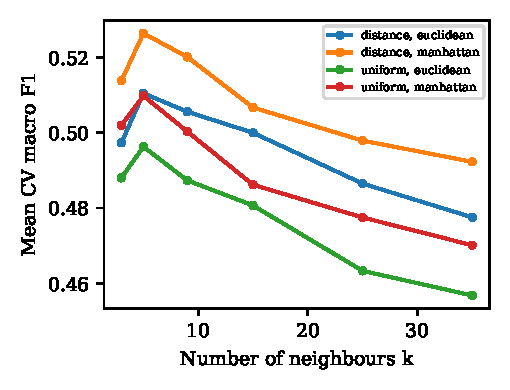
\includegraphics[width=0.95\linewidth]{../figures/knn_hyperparameter_search.pdf}
\caption{Mean cross-validated macro-averaged F1 score of k-nearest neighbours for every neighbourhood size, vote weighting scheme, and distance function evaluated during the control parameter search.}
\label{fig:knn-search}
\end{figure}

Figure~\ref{fig:tree-search} showed the corresponding score for the classification tree, for every combination of split criterion, maximum depth, and minimum leaf size evaluated during the search. The best configuration used the entropy split criterion, a maximum depth of twenty, and a minimum leaf size of one instance, reaching a score of 0.576. Performance improved sharply as the maximum depth increased from ten toward twenty, then declined gradually beyond a depth of twenty: a depth of twenty balanced the ability of the tree to separate the ten attack categories against the tendency of a deeper tree to overfit the training folds. A minimum leaf size of one instance and a minimum leaf size of five instances scored within 0.0003 of one another at every depth evaluated, so restricting every leaf to at least five instances cost negligible performance relative to leaving every leaf unrestricted. Minimum leaf sizes of twenty and fifty instances, by contrast, scored between 0.03 and 0.07 lower than a minimum leaf size of one at every depth evaluated: a sufficiently large minimum leaf size prevented the tree from capturing patterns specific to the least frequent attack categories.

\begin{figure}[t]
\centering
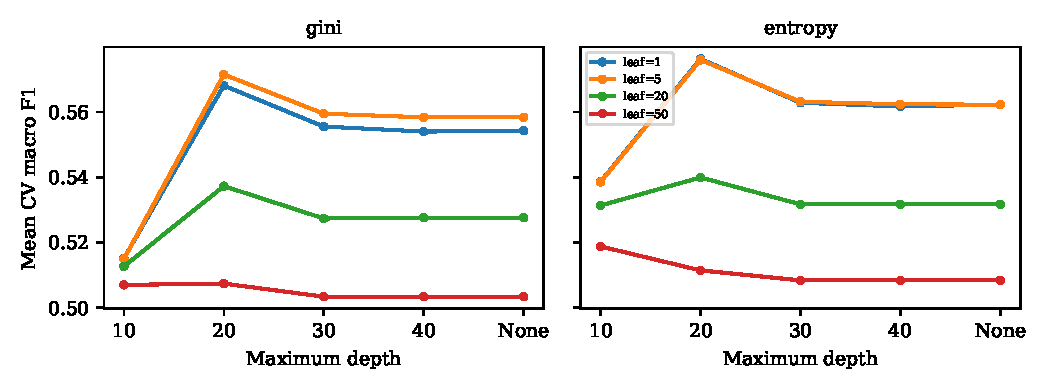
\includegraphics[width=0.95\linewidth]{../figures/tree_hyperparameter_search.pdf}
\caption{Mean cross-validated macro-averaged F1 score of the classification tree for every split criterion, maximum depth, and minimum leaf size evaluated during the control parameter search.}
\label{fig:tree-search}
\end{figure}

\subsection{Cross-Validated Performance}
\label{sec:results-cv}

Table~\ref{tab:performance} reported the mean and standard deviation of every performance measure in Section~\ref{sec:procedure-measures}, across the fifteen folds of the repeated cross-validation partition in Section~\ref{sec:procedure-cv}, for the selected configuration of each algorithm. K-nearest neighbours obtained a higher mean accuracy and a higher mean weighted-averaged F1 score than the classification tree. The classification tree obtained a higher mean macro-averaged F1 score and a higher mean balanced accuracy than k-nearest neighbours. Accuracy and the weighted-averaged F1 score were dominated by the two most frequent classes, normal and generic; these two classes together accounted for approximately 59 per cent of the instances. The higher accuracy of k-nearest neighbours therefore indicated superior performance on the frequent classes specifically, while the higher macro-averaged F1 score and balanced accuracy of the classification tree indicated superior performance when every class was weighted equally, including the least frequent classes.

\begin{table}[t]
\caption{Mean and standard deviation of cross-validated performance of k-nearest neighbours and the classification tree over fifteen repeated folds}
\label{tab:performance}
\centering
\footnotesize
\begin{tabular}{lcccc}
\toprule
Measure & kNN mean & kNN std & Tree mean & Tree std \\
\midrule
Accuracy & 0.802 & 0.001 & 0.759 & 0.005 \\
Macro F1 & 0.525 & 0.005 & 0.576 & 0.006 \\
Weighted F1 & 0.799 & 0.001 & 0.790 & 0.003 \\
Balanced acc. & 0.507 & 0.004 & 0.609 & 0.008 \\
\bottomrule
\end{tabular}
\end{table}

Figure~\ref{fig:comparison} presented the same mean performance values graphically, with error bars showing one standard deviation across the fifteen repeated folds. The Wilcoxon signed-rank test described in Section~\ref{sec:procedure-comparison} found the difference between the two algorithms statistically significant for all four performance measures, at the adopted significance level of 0.05: accuracy ($p=0.00006$), macro-averaged F1 score ($p=0.00006$), weighted-averaged F1 score ($p=0.00006$), and balanced accuracy ($p=0.00006$).

All four measures obtained the same p-value for a specific reason: in every one of the fifteen folds, the classification tree scored higher on accuracy, macro-averaged F1, weighted-averaged F1, and balanced accuracy than k-nearest neighbours, or lower on the measures that favoured k-nearest neighbours. This fully consistent ranking was the most extreme outcome obtainable from fifteen paired observations, and so gave the smallest p-value the test statistic could reach for a sample of this size. Table~\ref{tab:performance} also reported a consistently small standard deviation for every measure across the fifteen folds, showing that the performance of both algorithms was stable across different partitions of the data set. This stability corroborated the significant differences found by the Wilcoxon signed-rank test.

\begin{figure}[t]
\centering
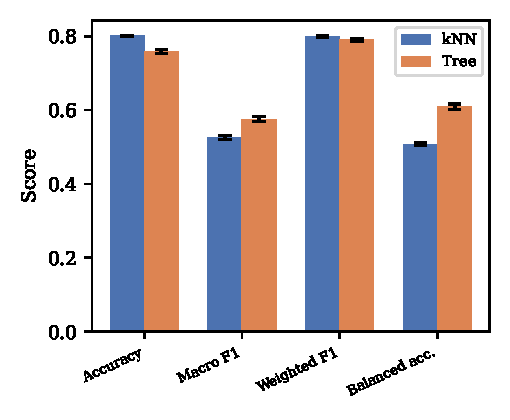
\includegraphics[width=0.95\linewidth]{../figures/model_comparison.pdf}
\caption{Mean cross-validated performance of k-nearest neighbours and the classification tree, with error bars indicating one standard deviation across the fifteen repeated folds.}
\label{fig:comparison}
\end{figure}

\subsection{Per-Class Performance}
\label{sec:results-perclass}

Figure~\ref{fig:perclass} showed the F1 score of the out-of-fold predictions for each of the ten attack categories, combining the predictions made when each fold in turn served as the test fold. Both algorithms scored above 0.88 for the normal category and above 0.98 for the generic category, the two most frequent categories. The classification tree scored substantially higher than k-nearest neighbours for the worms category, the least frequent category, at 0.596 against 0.209, and for the reconnaissance category, at 0.823 against 0.721: this illustrated the benefit of the class-weighted impurity criterion for the categories most affected by the skewed class distribution. K-nearest neighbours scored higher than the classification tree for the exploits category, at 0.681 against 0.649, and for the analysis category, at 0.186 against 0.098. Both algorithms scored low for the analysis and backdoor categories, at or below 0.19 and 0.09 respectively: neither algorithm reliably separated these two categories from the rest under the available descriptive features.

\begin{figure}[t]
\centering
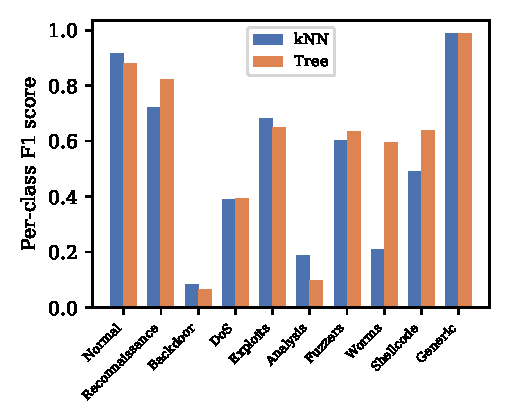
\includegraphics[width=0.95\linewidth]{../figures/per_class_f1.pdf}
\caption{Out-of-fold F1 score of k-nearest neighbours and the classification tree for every attack category.}
\label{fig:perclass}
\end{figure}

Figure~\ref{fig:cm-tree} and Figure~\ref{fig:cm-knn} showed the row-normalised confusion matrix of the out-of-fold predictions for the classification tree and k-nearest neighbours respectively. Every row sums to one and gives the distribution of predictions for the instances of the corresponding true category. Both matrices showed extensive mutual confusion between the backdoor, denial of service, and analysis categories: the classification tree most often predicted denial of service or analysis for backdoor instances, and k-nearest neighbours most often predicted exploits or denial of service. These three categories therefore shared overlapping descriptive feature values that neither algorithm separated reliably.

The two confusion matrices diverged most sharply for the worms category, the least frequent category in the data set. The classification tree correctly predicted worms for 63.2 per cent of worms instances. K-nearest neighbours correctly predicted worms for only 13.8 per cent of worms instances, and instead predicted exploits for 69.5 per cent of worms instances. This divergence matched the diagnostic check in Section~\ref{sec:methodology-impact-knn}: only 15.3 per cent of the nearest training neighbours of a sample of worms instances were themselves worms instances. The class-weighted impurity criterion of the classification tree reweighted the contribution of a worms instance directly during training. The distance-weighted voting of k-nearest neighbours only reweighted the influence of a neighbour already present in the neighbourhood of a query instance, and could not compensate for a neighbourhood where exploits instances outnumbered worms instances, regardless of distance.

\begin{figure}[t]
\centering
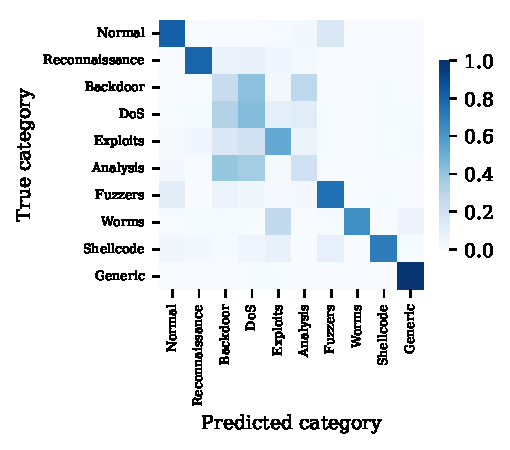
\includegraphics[width=0.85\linewidth]{../figures/tree_confusion_matrix.pdf}
\caption{Row-normalised confusion matrix of the out-of-fold predictions of the classification tree.}
\label{fig:cm-tree}
\end{figure}

\begin{figure}[t]
\centering
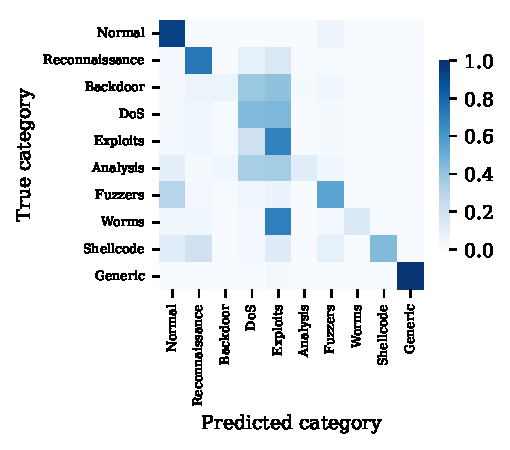
\includegraphics[width=0.85\linewidth]{../figures/knn_confusion_matrix.pdf}
\caption{Row-normalised confusion matrix of the out-of-fold predictions of k-nearest neighbours.}
\label{fig:cm-knn}
\end{figure}

Figure~\ref{fig:importance} showed the fifteen features the classification tree found most important, measured by the total reduction in impurity attributed to each feature across the complete tree fitted to the entire data set. The feature sbytes, the number of bytes transferred from source to destination, accounted for the largest share of impurity reduction, at 22.4 per cent. This was followed by the indicator for the dns value of the one-hot encoded feature service, at 15.9 per cent, the feature smean, at 11.1 per cent, and the connection-count feature ct\_dst\_src\_ltm, at 11.0 per cent. A second service indicator, for the http value, ranked at 4.2 per cent, and the indicator for the category created from the missing value symbol ranked at 1.6 per cent. The prominence of these service indicators confirmed that encoding the missing value symbol as a distinct category, described in Section~\ref{sec:methodology-prep-tree}, preserved information the classification tree found directly useful for separating the ten attack categories.

\begin{figure}[t]
\centering
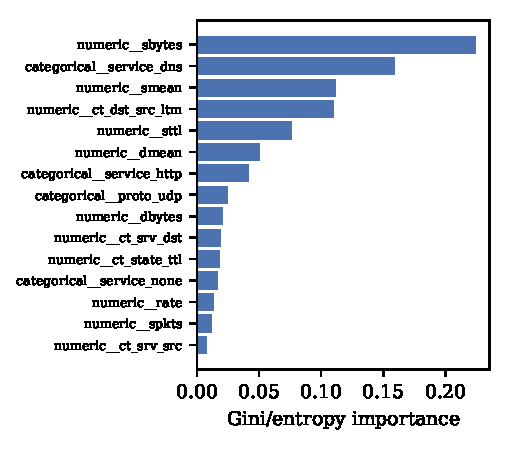
\includegraphics[width=0.95\linewidth]{../figures/tree_feature_importance.pdf}
\caption{Fifteen most important features of the classification tree, ranked by total impurity reduction.}
\label{fig:importance}
\end{figure}

\subsection{Discussion}
\label{sec:results-discussion}

The results in Section~\ref{sec:results-cv} and Section~\ref{sec:results-perclass} matched the expectations formed in Section~\ref{sec:methodology-impact-knn} and Section~\ref{sec:methodology-impact-tree}.

Section~\ref{sec:methodology-impact-knn} expected the skewed class distribution to bias k-nearest neighbours toward the frequent classes, since distance-weighted voting corrects for the relative closeness of the neighbours found, not for how frequently each class occurs among those neighbours. The low recall for the worms, backdoor, and shellcode categories, reported in Section~\ref{sec:results-perclass}, confirmed that distance weighting did not compensate for the skewed class distribution in Section~\ref{sec:methodology-dq}.

Section~\ref{sec:methodology-impact-tree} expected the class-weighted impurity criterion to protect the least frequent categories more directly than distance weighting, since the criterion applies during training, not only at the point of prediction. The substantially higher recall of the classification tree for the worms category, shown in Figure~\ref{fig:cm-tree} and Figure~\ref{fig:cm-knn}, confirmed this expectation.

The two algorithms nevertheless remained close in overall accuracy and weighted-averaged F1 score. Both measures were dominated by the normal and generic categories; neither algorithm found these two categories difficult to separate from the rest. This similarity explained why the Wilcoxon signed-rank test found a significant difference in accuracy favouring k-nearest neighbours, alongside a significant difference in macro-averaged F1 score and balanced accuracy favouring the classification tree.

The classification tree was the more suitable algorithm for the attack category prediction task addressed in this report. This conclusion rested primarily on the macro-averaged F1 score and the balanced accuracy of the classification tree: both measures treated every attack category equally, rather than being dominated by the frequent categories. A network intrusion detection system that fails to detect a rare but severe attack category, such as worms or backdoors, causes greater practical harm than a system that occasionally misclassifies a common, largely benign traffic pattern. The accuracy measure, where k-nearest neighbours scored marginally higher, therefore did not outweigh the balanced accuracy of 0.609 for the classification tree against 0.507 for k-nearest neighbours.

The shorter pre-processing pipeline required for the classification tree, described in Section~\ref{sec:methodology-prep-tree}, reinforced the conclusion. The classification tree reached superior performance on the primary measures without the log transformation, the standardisation, or the correlated feature removal that the k-nearest neighbours pipeline required.

\section{Conclusion}
\label{sec:conclusion}

This report developed and compared two classification models, k-nearest neighbours (kNN) and a classification tree, for predicting the attack category of a network flow in a version of the UNSW-NB15 network traffic data set.

Exploratory analysis found a substantial proportion of missing values in one feature, several pairs of near-perfectly correlated features, large positive outliers in most numeric features, numeric features on widely different scales, and three nominal categorical features, one with high cardinality. One feature had values outside the range implied by the data set documentation. Investigation, rather than correction on the assumption that a range violation is always an error, showed this feature agrees with an independently recorded feature on 99.997 per cent of the instances, so no correction was warranted.

The pre-processing pipelines confirmed the expected pattern: feature scale, outlying values, and feature correlation matter for a distance-based classifier such as kNN, but not for a threshold-based classifier such as a classification tree. The missing values in one feature, and the unique record identifier, required correction regardless of the classification algorithm applied afterward. Two pre-processing pipelines were built accordingly: one addressing every issue relevant to kNN as a distance-based classifier, and a considerably shorter pipeline for the classification tree that corrected only the issues present in the content of the data set, leaving untouched the issues of scale, outlying values, and feature correlation that a threshold-based classifier tolerates without a dedicated transformation.

Under repeated stratified cross-validation (CV), the classification tree reached a mean macro-averaged F1 score of 0.576 and a mean balanced accuracy of 0.609, above the corresponding mean scores of 0.525 and 0.507 for k-nearest neighbours. The Wilcoxon signed-rank test found this margin statistically significant. K-nearest neighbours reached a marginally higher mean accuracy, 0.802 against 0.759 for the classification tree.

The classification tree is the more suitable algorithm for the network intrusion detection task addressed in this report. The macro-averaged F1 score and the balanced accuracy, the two measures that treat every attack category equally rather than being dominated by the most frequent categories, both favour the classification tree. A network intrusion detection system also benefits more from reliably detecting a rare, severe attack category than from a marginal accuracy gain driven by categories already well separated by both algorithms.

The distance-weighted voting scheme applied for k-nearest neighbours corrects for the proximity of the training neighbours of a query instance, but not for how frequently each class occurs among those neighbours. This scheme therefore does not protect the least frequent attack categories to the same extent as the class-weighted training criterion of the classification tree.

This study is subject to limitations that constrain the generality of the conclusions. The control parameter search in Section~\ref{sec:procedure-hyperparameters} evaluated a bounded grid of candidate values for each algorithm, using a single stratified five-fold partition. A configuration outside this grid, for example a neighbourhood size for k-nearest neighbours beyond the largest value searched, was not considered and might give a different outcome; a different five-fold partition might also select a different configuration as optimal.

Future work could extend the comparison to further classification algorithms evaluated under the same pre-processing and empirical procedure. Future work could also investigate a resampling-based treatment of class imbalance, for example the synthetic minority over-sampling technique proposed by Chawla et al.~\cite{chawla2002}, as an alternative to the distance weighting and the class-weighted impurity criterion applied here for k-nearest neighbours and the classification tree respectively.

\appendix

\section*{Appendix A: List of Acronyms}
\begin{tabular}{ll}
CV & cross-validation \\
kNN & k-nearest neighbours \\
\end{tabular}

\section*{Appendix B: List of Symbols}
\begin{tabular}{@{}lp{0.36\textwidth}@{}}
$d(\cdot,\cdot)$ & the Minkowski distance function of Equation~\eqref{eq:minkowski} \\
$g(t)$ & the Gini index of node $t$ of a classification tree \\
$h(t)$ & the entropy of node $t$ of a classification tree \\
$k$ & the neighbourhood size control parameter of k-nearest neighbours \\
$m$ & the total number of classes in the target feature \\
$p$ & the order of the Minkowski distance of Equation~\eqref{eq:minkowski} \\
$p_{t,c}$ & the proportion of instances at node $t$ belonging to class $c$ \\
$t$ & a node of a classification tree \\
$\mathbf{x}_i$ & the feature vector of instance $i$ \\
$x_{i,l}$ & the value of the $l$-th feature of instance $i$ \\
\end{tabular}

\begin{thebibliography}{9}

\bibitem{aggarwal2001}
C.~C. Aggarwal, A.~Hinneburg, and D.~A. Keim, ``On the surprising behavior of distance metrics in high dimensional space,'' in \emph{Proceedings of the International Conference on Database Theory}, Lecture Notes in Computer Science, vol.~1973. Berlin, Germany: Springer, 2001, pp. 420--434.

\bibitem{breiman1984}
L.~Breiman, J.~H. Friedman, R.~A. Olshen, and C.~J. Stone, \emph{Classification and Regression Trees}. Belmont, CA: Wadsworth, 1984.

\bibitem{chawla2002}
N.~V. Chawla, K.~W. Bowyer, L.~O. Hall, and W.~P. Kegelmeyer, ``SMOTE: synthetic minority over-sampling technique,'' \emph{Journal of Artificial Intelligence Research}, vol.~16, pp. 321--357, 2002.

\bibitem{cover1967}
T.~Cover and P.~Hart, ``Nearest neighbor pattern classification,'' \emph{IEEE Transactions on Information Theory}, vol.~13, no.~1, pp. 21--27, 1967.

\bibitem{hodge2004}
V.~J. Hodge and J.~Austin, ``A survey of outlier detection methodologies,'' \emph{Artificial Intelligence Review}, vol.~22, no.~2, pp. 85--126, 2004.

\bibitem{kelleher2020}
J.~D. Kelleher, B.~Mac Namee, and A.~D'Arcy, \emph{Fundamentals of Machine Learning for Predictive Data Analytics: Algorithms, Worked Examples, and Case Studies}, 2nd~ed. Cambridge, MA: MIT Press, 2020.

\bibitem{kohavi1995}
R.~Kohavi, ``A study of cross-validation and bootstrap for accuracy estimation and model selection,'' in \emph{Proceedings of the International Joint Conference on Artificial Intelligence}, vol.~14, 1995, pp. 1137--1143.

\bibitem{moustafa2015}
N.~Moustafa and J.~Slay, ``UNSW-NB15: a comprehensive data set for network intrusion detection systems,'' in \emph{Proceedings of the Military Communications and Information Systems Conference}, Canberra, Australia, 2015, pp. 1--6.

\bibitem{quinlan1986}
J.~R. Quinlan, ``Induction of decision trees,'' \emph{Machine Learning}, vol.~1, no.~1, pp. 81--106, 1986.

\bibitem{rainio2024}
O.~Rainio, J.~Teuho, and R.~Klén, ``Evaluation metrics and statistical tests for machine learning,'' \emph{Scientific Reports}, vol.~14, article 6086, 2024.

\bibitem{shepard1968}
D.~Shepard, ``A two-dimensional interpolation function for irregularly-spaced data,'' in \emph{Proceedings of the ACM National Conference}, New York, NY, 1968, pp. 517--524.

\end{thebibliography}

\end{document}
